\documentclass{article}
\usepackage[utf8]{inputenc}
\usepackage{tikz}
\usepackage{amsmath}

\title{Assignment4}
\author{Swapnil Sirsat}
\date{January 2021}

\begin{document}
\maketitle
\section*{Question: }
Draw $\Delta$ABC with a = 7, $\angle$B = 45$^\circ$
and $\angle$A = 105$^\circ$
\section*{Answer: }
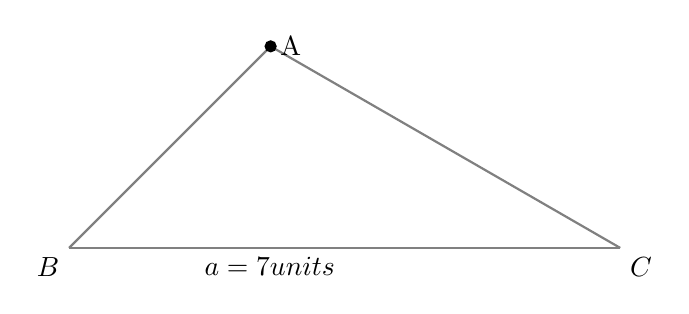
\begin{tikzpicture}
\draw[gray, thick](0,0) -- (7,0);
\draw[gray, thick](0,0) -- (2.56,2.56);
\draw[gray, thick](7,0) -- (2.56,2.56);
\node at(0,0)[below left]{$B$};
\node at(3.5,0)[below left]{$a = 7units$};
\node at(7,0)[below right]{$C$};
\filldraw[black] (2.56,2.56) circle (2pt) node[anchor=west] {A};
\end{tikzpicture}\\
To construct $\Delta$ABC we first need to find $\angle$C\\
By angle sum property we know that
\begin{align}
    \angle A + \angle B + \angle C = 180^\circ
\end{align}
putting values of $\angle$A and $\angle$B in equation 1 we get
\begin{gather*}
    45^\circ + 105^\circ + \angle C = 180^\circ\\
        \angle C = 180^\circ - 150^\circ \\
        \angle C = 30^\circ
\end{gather*}
Now,
\begin{gather*}
    \angle B = 45^\circ\\
    \angle C = 30^\circ 
\end{gather*}
therefore, line BA and CA would be as 
\begin{gather}
    x = y         \mbox{     \hspace{2cm} (as B is at (0 , 0 ))} \\
    y = \frac{-1}{\sqrt{3}}(x - 7 ) \mbox{\hspace{2cm} (C is at (0,7)) }
\end{gather}
therefore the point of intersection of the two lines by substitution equation 2 in 3
\begin{gather*}
    y = \frac{-1}{\sqrt{3}} (y - 7) \\
    y + \frac{1}{\sqrt{3}} y = \frac{7}{\sqrt{3}} \\
    y =\frac{\frac{7}{\sqrt{3}}}{1+\frac{1}{\sqrt{3}}} \\
    y = 2.56\\
    \implies x = 2.56
\end{gather*}
therefore the coordinates for the triangle taking B at origin would be as
\begin{gather*}
    A = (2.56,2.56)\\
    B = (0, 0) \\
    C = (0 , 7)\\
\end{gather*}
the constructed figure through matplotlib in python would be as:
\begin{figure}[h!]
    \centering
    \includegraphics[height = 200]{code.PNG}
    \caption{$\Delta$ABC}
    \label{fig:my_label}
\end{figure}


\end{document}
